% Artigo no modelo da revista Linguamática (template da disciplina de PLN, Ibmec BH, 2026/02).
% Overleaf: envie main.tex, referencias.bib e a pasta figuras/ para o projeto do template
% (que já contém linguamatica.sty e sp_por.bst) e substitua o main.tex de exemplo.
% Se o preâmbulo do projeto do professor for diferente deste, mantenha o dele e cole daqui
% só o conteúdo entre \begin{document} e \end{document}.
% Números: resultados/tabelas/ (gerados por `python -m fakebr.relatorio`).
% \conferir{...} marca afirmações sobre trabalhos de terceiros a confirmar na fonte (sai em vermelho).
\documentclass[a4paper, twocolumn, 11pt, twoside]{article}

\usepackage[utf8]{inputenc}
\usepackage[T1]{fontenc}
\usepackage[portuges]{babel}
\usepackage{linguamatica}
\usepackage{natbib}          % já carregado pelo linguamatica.sty na maioria das versões; repetir não tem efeito
\usepackage{graphicx}
\usepackage{booktabs}
\usepackage{xcolor}
\usepackage{adjustbox}       % encolhe tabelas largas até caberem na coluna/página (nunca amplia)

\newcommand{\conferir}[1]{\textcolor{red}{[conferir: #1]}}

\title{Atalhos de Fonte e de Formatação na Detecção\\de Notícias Falsas em Português}
\titleEN{Source and Formatting Shortcuts in Portuguese Fake News Detection}

% Sintaxe do exemplo oficial: nome, \instituto{...} e \email{...}, autores separados por \and.
% Se o template do professor tiver o ORCID no bloco dele, copie aquela linha para cá.
\author{
  Lucas Mendes Buccini
  \instituto{Ibmec BH}
  \email{lucasmbuccini@gmail.com}
\and
  Eduardo Campos dos Santos
  \instituto{Ibmec BH}
  \email{edu.campos.santos@gmail.com}
}

\begin{document}

\maketitle

\begin{resumo}
Comparamos, sob um protocolo único, quatro famílias de classificadores para detectar notícias falsas em português no Fake.Br: modelos estatísticos sobre TF-IDF, embeddings congelados, o BERTimbau com ajuste fino e um LLM de pesos abertos (Qwen2.5-7B) por aprendizado no contexto. Antes de comparar modelos, quantificamos três atalhos do corpus: nos textos completos, só o tamanho dá 94,2\% de acurácia; na versão de tamanho normalizado, o truncamento deixa 93\% das notícias verdadeiras terminando no meio de uma frase, e quatro marcas de formatação bastam para 83,1\%; e 93\% das falsas vêm de um único site. Nos textos normalizados, a SVM sobre palavras atinge 91,7\%, n-gramas de caracteres 94,6\%, embeddings congelados do BERTimbau 95,7\%, o BERTimbau ajustado 99,5\% e o LLM 78,4\% (few-shot calibrado). Com os artefatos de formatação neutralizados, o BERTimbau ajustado mantém 98,7\% e é o único modelo que generaliza para as fontes minoritárias. A avaliação no Fake.Br precisa controlar tamanho, formatação e fonte para que os números signifiquem detecção de desinformação.
\end{resumo}
\palavraschave{notícias falsas, classificação de textos, BERTimbau, LLM, aprendizado por atalhos}

\begin{abstract}
We compare, under a single protocol, four families of classifiers for Portuguese fake news detection on Fake.Br: TF-IDF statistical models, frozen embeddings, fine-tuned BERTimbau, and an open-weight LLM (Qwen2.5-7B) with in-context learning. Before comparing models, we quantify three corpus shortcuts: on full texts, length alone yields 94.2\% accuracy; in the size-normalized version, truncation leaves 93\% of true articles ending mid-sentence and four formatting cues reach 83.1\%; and 93\% of fake articles come from a single website. On normalized texts, a word-level SVM reaches 91.7\%, character n-grams 94.6\%, frozen BERTimbau 95.7\%, fine-tuned BERTimbau 99.5\%, and the LLM 78.4\% (calibrated few-shot). With formatting artifacts neutralized, fine-tuned BERTimbau keeps 98.7\% and is the only model that generalizes to minority sources. Evaluation on Fake.Br must control for length, formatting, and source for the numbers to reflect misinformation detection.
\end{abstract}
\keywords{fake news, text classification, BERTimbau, LLM, shortcut learning}

% ============================================================================================
\section{Introdução}

A circulação de notícias falsas em ambientes digitais tornou-se um problema de interesse público, com efeitos sobre processos eleitorais, campanhas de saúde e a confiança no jornalismo \citep{shu2017,zhou2020}. No Brasil, onde redes sociais e aplicativos de mensagens estão entre as principais fontes de informação, esse conteúdo se espalha mais rápido do que as agências de checagem conseguem verificá-lo. Ferramentas de triagem automática podem reduzir esse descompasso, mas a maior parte dos recursos e resultados comparativos foi produzida para o inglês.

O Fake.Br \citep{monteiro2018} é o principal corpus anotado para a tarefa em português. Este trabalho compara nele modelos de complexidade crescente, de uma linha de base estatística barata e interpretável até um modelo de linguagem de propósito geral, para medir quanto cada aumento de custo efetivamente rende. Ao longo da comparação, verificamos que parte importante do desempenho pode vir de regularidades do corpus sem relação com a veracidade: o tamanho dos textos, marcas de formatação criadas pela própria normalização de tamanho e a concentração das notícias falsas num único site. Esse fenômeno, o aprendizado por atalhos \citep{geirhos2020}, muda a leitura dos resultados e tornou-se o segundo eixo do trabalho.

As contribuições são: (i)~um protocolo de avaliação reprodutível para o Fake.Br, com partição por pares, seleção de hiperparâmetros por validação cruzada agrupada, intervalos de confiança por \emph{bootstrap} de pares e testes pareados com correção para comparações múltiplas; (ii)~a comparação de quatro famílias de modelos sob esse protocolo; e (iii)~a quantificação de três atalhos do corpus, com um pré-processamento que neutraliza os artefatos de formatação e análises por subgrupo que medem quanto cada modelo depende deles.

% ============================================================================================
\section{Trabalhos Relacionados}

\paragraph{Fake.Br.} \citet{monteiro2018} construíram o corpus e obtiveram cerca de 89\% de F1 com SVM sobre a versão de tamanho normalizado \conferir{valor e atributos}. \citet{silva2020} ampliaram a avaliação com diversas representações e classificadores \conferir{melhores resultados}. Ambos já apontavam a diferença de tamanho entre as classes, razão da versão normalizada.

\paragraph{Classificação clássica de textos.} TF-IDF \citep{salton1988} com SVM linear \citep{joachims1998} ou Naive Bayes Multinomial \citep{mccallum1998} é uma linha de base forte em espaços esparsos de alta dimensionalidade, com treino em segundos e pesos interpretáveis.

\paragraph{Transformers para o português.} O BERTimbau \citep{souza2020} é um BERT \citep{devlin2019} pré-treinado no corpus brWaC e é a referência para classificação em português brasileiro. Codificadores multilíngues de sentenças, como o Multilingual-E5 \citep{wang2024e5}, permitem usar representações contextuais sem ajuste fino.

\paragraph{LLMs por aprendizado no contexto.} Modelos de linguagem grandes resolvem tarefas a partir de instruções e poucos exemplos \citep{brown2020}, mas são sensíveis ao \emph{prompt} e tendem a preferir certas respostas, viés que a calibração contextual corrige em parte \citep{zhao2021}. A contaminação dos dados de avaliação no pré-treinamento é uma ressalva conhecida \citep{sainz2023}, e a quantização em 4 bits \citep{dettmers2023} permite executá-los em GPUs de 16~GB.

\paragraph{Atalhos e artefatos.} Modelos tendem a explorar a regra mais simples que separa os dados de treino, mesmo quando ela não corresponde à tarefa pretendida \citep{geirhos2020}. Em PLN, artefatos de construção dos dados permitiram, por exemplo, resolver inferência textual olhando só a hipótese \citep{gururangan2018}.

% ============================================================================================
\section{Corpus}

O Fake.Br \citep{monteiro2018} reúne 7\,200 notícias em português brasileiro publicadas entre 2016 e 2018: 3\,600 falsas e 3\,600 verdadeiras. Cada notícia falsa foi alinhada manualmente a uma verdadeira sobre o mesmo assunto, formando 3\,600 pares, em seis categorias: política (58\%), TV e celebridades (21\%), sociedade e cotidiano (18\%), ciência e tecnologia (1,6\%), economia e religião (0,6\% cada).

\subsection{Viés de tamanho}

Nos textos completos, a notícia verdadeira é mais longa que a falsa em 98,2\% dos pares, com razão mediana de 6,1 entre os tamanhos (Tabela~\ref{tab:tamanho}, Figura~\ref{fig:tamanho}). Os autores disponibilizam uma versão de tamanho normalizado, na qual o texto mais longo de cada par é truncado ao número de palavras do mais curto; nela, a razão mediana cai para 1,01. Todos os experimentos principais usam essa versão.

\begin{table}[t]
\centering\small
\begin{adjustbox}{max width=\columnwidth}
\begin{tabular}{llrrr}
\toprule
Versão & Classe & Média & Mediana & Máx. \\
\midrule
Completa & Falsa & 185,9 & 157 & 2\,288 \\
Completa & Verdadeira & 1\,100,3 & 918 & 7\,517 \\
Normalizada & Falsa & 182,8 & 157 & 2\,088 \\
Normalizada & Verdadeira & 184,3 & 158 & 2\,095 \\
\bottomrule
\end{tabular}
\end{adjustbox}
\caption{Palavras por notícia, por classe e versão do corpus.}
\label{tab:tamanho}
\end{table}

\begin{figure*}[t]
\centering
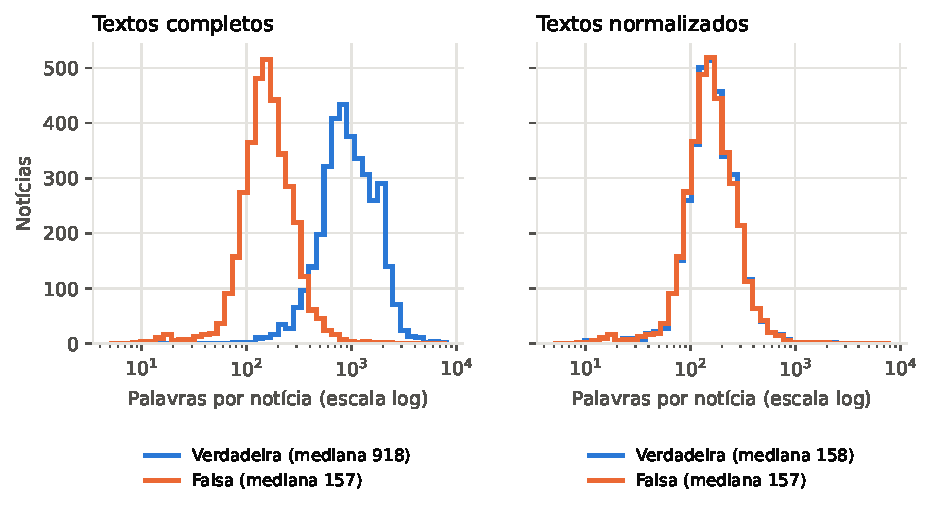
\includegraphics[width=0.9\textwidth]{figuras/distribuicao_tamanho.pdf}
\caption{Distribuição do número de palavras por classe nas duas versões do corpus.}
\label{fig:tamanho}
\end{figure*}

\subsection{Artefatos de formatação da normalização}

A normalização corrige o tamanho, mas cria outro sinal. Como o texto truncado é quase sempre o verdadeiro, ele termina no meio de uma frase: na versão normalizada, \textbf{70,4\% das notícias falsas terminam com pontuação final, contra 6,7\% das verdadeiras}. Há ainda diferenças de formatação entre os sites: aspas retas aparecem em 80,8\% das falsas e 32,4\% das verdadeiras, aspas tipográficas em 4,8\% e 23,2\%, e a sequência ``. .'' separando título e corpo em 25,0\% e 10,6\%. Nenhuma dessas marcas diz respeito à veracidade.

\subsection{Concentração das fontes}

As notícias falsas vêm de apenas seis sites, e \textbf{3\,335 das 3\,600 (92,6\%) de um único domínio} (diariodobrasil.org); as verdadeiras vêm de 25 domínios, com predominância do G1 e do Estadão. Um classificador pode, assim, aprender o estilo editorial de um site em vez de marcas gerais de desinformação. No teste, apenas 44 notícias falsas vêm de outras fontes.

\subsection{Qualidade dos dados}

As duas versões não têm a mesma numeração de pares: a completa não tem os pares 697 e 1468, a normalizada não tem os pares 586 e 1607, e ambas vão até 3602. Verificamos que o número N corresponde à mesma notícia nas duas versões, de modo que os metadados (categoria, fonte, data) da versão completa valem para a normalizada, exceto em dois pares sem metadados.

% ============================================================================================
\section{Metodologia}

\subsection{Particionamento}

Os 3\,600 pares da versão normalizada foram sorteados uma única vez (semente 42) em treino, validação e teste, na proporção 70/15/15: 5\,040, 1\,080 e 1\,080 notícias, metade de cada classe em cada parte. A unidade sorteada é o par, de modo que o tema de uma notícia de teste nunca é visto no treino por meio da sua contraparte. O treino ajusta os modelos e escolhe hiperparâmetros; a validação escolhe o ponto de parada do BERTimbau e o limiar do LLM; o teste é usado uma única vez.

\subsection{Pré-processamento}

Usamos três configurações, implementadas como \emph{pipelines} declarativos e serializáveis:
\begin{itemize}
\item \textbf{Completo} (saco de palavras): remoção de HTML, URLs e e-mails; minúsculas; remoção de números e pontuação; tokenização por expressão regular; remoção de \emph{stopwords} (NLTK); descarte de tokens com menos de dois caracteres. Radicalização RSLP \citep{orengo2001} e lematização (spaCy) entram como ablação.
\item \textbf{Mínimo} (n-gramas de caracteres, Transformers e LLM): apenas remoção de HTML, URLs e e-mails e normalização de espaços.
\item \textbf{Neutro} (controle dos artefatos): o mínimo, mais a padronização das aspas, a troca de ``. .'' por um ponto, o corte de todo texto na última frase completa e a remoção da pontuação final. Nenhuma notícia, de nenhuma classe, termina em frase interrompida ou com marca de fim.
\end{itemize}
O pré-processamento completo já remove toda a pontuação, de modo que os modelos sobre palavras são imunes aos artefatos de formatação.

\subsection{Modelos}

\paragraph{Experimento 0: atalhos.} Regressões Logísticas que não leem o conteúdo: com o logaritmo do número de palavras e de caracteres (versões completa, normalizada e neutra) e com quatro indicadores de formatação (termina com pontuação final, contém aspas retas, contém aspas tipográficas, contém ``. .''), nas versões mínima e neutra.

\paragraph{Experimento 1: modelos estatísticos.} TF-IDF de unigramas e bigramas (\texttt{min\_df}~=~2, \texttt{max\_df}~=~0,95, tf sublinear) com Naive Bayes Multinomial, SVM linear e Regressão Logística. Ablações sobre a SVM mudam uma decisão por vez: manter \emph{stopwords}, radicalização, lematização, só unigramas e n-gramas de caracteres (2 a 5) com pré-processamento mínimo e neutro. A regularização é escolhida por busca em grade com validação cruzada de 5 dobras no treino, agrupada por par; o TF-IDF é ajustado dentro de cada dobra.

\paragraph{Experimento 2: embeddings congelados.} Vetores do BERTimbau Base sem ajuste fino (média dos vetores da última camada) e do Multilingual-E5 Base \citep{wang2024e5}, até 512 subpalavras, seguidos de padronização e Regressão Logística.

\paragraph{Experimento 3: BERTimbau ajustado.} BERTimbau Base (110~M de parâmetros) com uma camada de classificação sobre o token \texttt{[CLS]} e todos os pesos ajustados: AdamW, taxa $2\times10^{-5}$ com decaimento linear e 10\% de aquecimento, \emph{weight decay} 0,01, lote efetivo 16, 4 épocas, bf16, entradas truncadas em 512 subpalavras (4,4\% dos textos de teste excedem o limite). O melhor ponto na validação é restaurado. Usamos três sementes (42, 13 e 7), nos textos mínimo e neutro.

\paragraph{Experimento 4: LLM.} Qwen2.5-7B-Instruct \citep{qwen2025}, quantizado em 4 bits (NF4) \citep{dettmers2023}, sem atualização de pesos. O \emph{prompt} de sistema descreve a tarefa em português e pede uma única palavra, FALSA ou VERDADEIRA; no \emph{few-shot}, quatro exemplos do treino (dois de cada classe, de pares distintos) entram como turnos anteriores do diálogo. Em vez de gerar texto, usamos como escore $\log P(\textrm{FALSA}) - \log P(\textrm{VERDADEIRA})$ no próximo token, o que elimina respostas fora do formato e fornece um escore contínuo. Há duas regras de decisão: limiar zero e limiar escolhido na validação, uma calibração contextual simples \citep{zhao2021}. Notícias são truncadas em 400 palavras e exemplos em 150.

\subsection{Avaliação}

A métrica principal é a acurácia, adequada às classes balanceadas; reportamos também precisão, revocação e F1 da classe falsa e ROC-AUC. Os intervalos de confiança de 95\% vêm de \emph{bootstrap} percentil \citep{efron1993} com 2\,000 reamostras \textbf{de pares}, já que as duas notícias de um par não são independentes. Modelos são comparados pelo teste exato de McNemar \citep{dietterich1998} com correção de \citet{holm1979}. A dependência dos atalhos é medida no texto neutro e por subgrupos de fonte e de final do texto. Os experimentos rodaram numa GPU NVIDIA RTX 2000 Ada (16~GB) e numa CPU de 20 \emph{threads}.

% ============================================================================================
\section{Resultados}

\begin{table*}[t]
\centering\small
\begin{adjustbox}{max width=\textwidth}
\begin{tabular}{llcccc}
\toprule
Família & Modelo & Acurácia & IC 95\% & F1 & ROC-AUC \\
\midrule
0. Atalhos & TF-IDF + SVM, textos completos & 97,1 & [96,0; 98,1] & 97,1 & 0,997 \\
 & Só tamanho, textos completos & 94,2 & [92,7; 95,6] & 94,2 & 0,981 \\
 & Só tamanho, normalizados & 56,4 & [53,3; 59,2] & 55,4 & 0,598 \\
 & Só formatação, normalizados & 83,1 & [80,6; 85,3] & 81,4 & 0,909 \\
 & Só formatação, neutro & 66,7 & [64,3; 69,2] & 71,3 & 0,667 \\
\midrule
1. Clássicos & TF-IDF + Naive Bayes & 88,4 & [86,7; 90,2] & 88,2 & 0,950 \\
 & TF-IDF + Regressão Logística & 91,4 & [89,8; 93,0] & 91,4 & 0,973 \\
 & TF-IDF + SVM linear & 91,7 & [90,0; 93,2] & 91,7 & 0,972 \\
 & n-gramas de caracteres + SVM & 94,6 & [93,2; 95,9] & 94,5 & 0,987 \\
\midrule
2. Congelados & Multilingual-E5 + RegLog & 91,2 & [89,6; 92,9] & 91,2 & 0,975 \\
 & BERTimbau + RegLog & 95,7 & [94,4; 96,9] & 95,7 & 0,993 \\
\midrule
3. Ajuste fino & BERTimbau (3 sementes) & 99,5 $\pm$ 0,1 & -- & 99,5 $\pm$ 0,1 & 1,000 \\
\midrule
4. LLM & Qwen2.5-7B \emph{zero-shot}, limiar 0 & 69,6 & [67,5; 71,9] & 59,2 & 0,832 \\
 & Qwen2.5-7B \emph{zero-shot}, calibrado & 75,6 & [73,2; 78,1] & 76,1 & 0,832 \\
 & Qwen2.5-7B \emph{few-shot}, limiar 0 & 76,4 & [74,0; 78,9] & 74,0 & 0,855 \\
 & Qwen2.5-7B \emph{few-shot}, calibrado & 78,4 & [76,2; 80,8] & 77,9 & 0,855 \\
\bottomrule
\end{tabular}
\end{adjustbox}
\caption{Desempenho no teste (1\,080 notícias), em \%. F1 da classe falsa; IC 95\% por \emph{bootstrap} de pares; BERTimbau ajustado: média $\pm$ desvio-padrão em três sementes.}
\label{tab:resultados}
\end{table*}

\begin{figure*}[t]
\centering
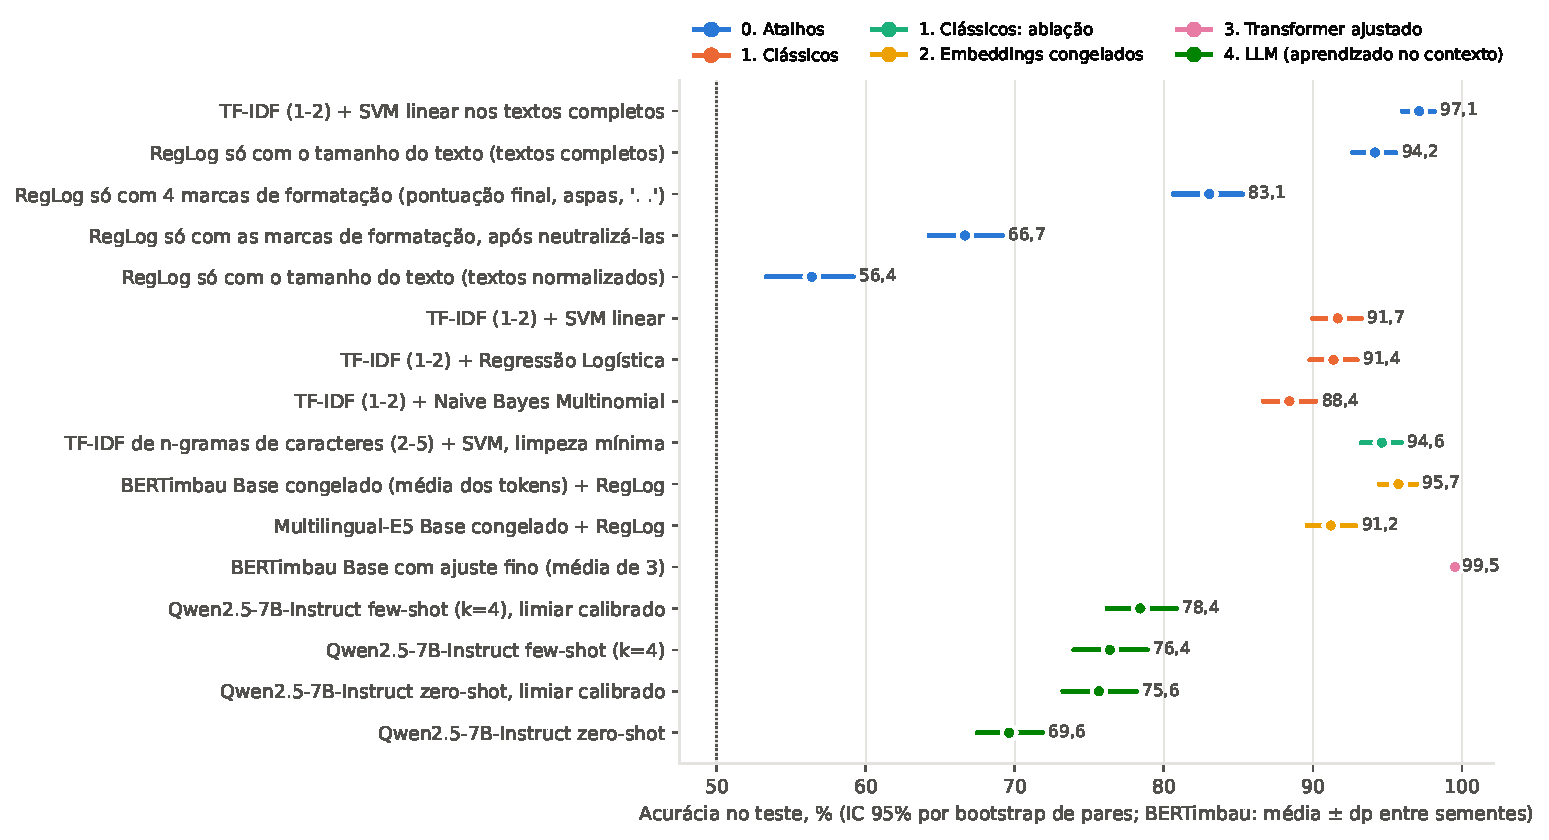
\includegraphics[width=0.9\textwidth]{figuras/comparacao_acuracia_artigo.pdf}
\caption{Acurácia no teste por modelo, com IC 95\% por \emph{bootstrap} de pares (modelos com várias sementes: média $\pm$ desvio-padrão).}
\label{fig:acuracia}
\end{figure*}

\subsection{Atalhos}

Só com o tamanho do texto, uma Regressão Logística acerta 94,2\% das notícias completas, e a SVM sobre TF-IDF chega a 97,1\% (Tabela~\ref{tab:resultados}). Na versão normalizada, o tamanho sozinho cai para 56,4\%, mas quatro indicadores de formatação, sem nenhuma palavra do texto, chegam a 83,1\%. Depois da neutralização, o tamanho continua sem informação (56,9\%) e a formatação cai para 66,7\%; o que resta é o uso de aspas, que reflete o hábito de citar e é um traço de estilo legítimo.

\subsection{Modelos estatísticos}

SVM linear (91,7\%) e Regressão Logística (91,4\%) são equivalentes e superam o Naive Bayes (88,4\%; McNemar, $p$ ajustado $< 0{,}001$), em linha com \citet{monteiro2018} \conferir{valor}. Nenhuma normalização morfológica ajudou: radicalização (90,1\%) e lematização (89,7\%) ficaram abaixo da SVM sem normalização, e manter as \emph{stopwords} não mudou o resultado (91,9\%). A maior melhora veio dos n-gramas de caracteres com pré-processamento mínimo (94,6\%; $p$ ajustado $< 0{,}001$ contra a SVM sobre palavras), ganho que não vem dos artefatos: no texto neutro eles mantêm 93,9\%.

Entre os termos de maior peso da SVM, os associados às verdadeiras são convenções do jornalismo profissional (``nesta terça'', ``quarta-feira'', ``segundo''); do lado das falsas aparecem nomes de políticos, verbos de relato (``disse'', ``declarou'') e marcas de registro como ``pra'' e ``coréia'', grafia anterior ao Acordo Ortográfico, enquanto as verdadeiras usam ``coreia''. São indícios de que o modelo captura o estilo editorial das fontes, e não a veracidade.

\subsection{Representações contextuais e ajuste fino}

Os embeddings congelados do BERTimbau (95,7\%) superam a SVM sobre palavras ($p$ ajustado $< 0{,}001$) e empatam com os n-gramas de caracteres ($p$ ajustado $= 0{,}28$); o Multilingual-E5 (91,2\%) fica no nível do TF-IDF, indicando que o pré-treinamento em português importa mais que o treinamento para similaridade. O ajuste fino leva o BERTimbau a 99,5\% $\pm$ 0,1 (99,6\%, 99,5\% e 99,4\% nas três sementes), com 4 a 6 erros em 1\,080 notícias, superando todos os demais modelos ($p$ ajustado $< 10^{-10}$).

\subsection{LLM por aprendizado no contexto}

O Qwen2.5-7B fica bem abaixo de todos os modelos treinados: 69,6\% em \emph{zero-shot} com limiar zero. O modelo tem um viés forte para a resposta VERDADEIRA: com limiar zero, chama de falsas apenas 264 das 1\,080 notícias (precisão 90,2\%, revocação 44,1\%), e o limiar ótimo na validação é $-9{,}9$ em log-odds. A calibração do limiar corrige esse viés e leva o \emph{zero-shot} a 75,6\%. Os quatro exemplos do \emph{few-shot} reduzem o viés (limiar ótimo $-2{,}3$) e elevam a ROC-AUC de 0,832 para 0,855; com calibração, o \emph{few-shot} chega a 78,4\%, diferença não significativa em relação ao \emph{zero-shot} calibrado ($p$ ajustado $= 0{,}059$). Mesmo calibradas, as duas versões ficam abaixo do Naive Bayes ($p$ ajustado $< 10^{-9}$). O custo é o mais alto de todos: cerca de 0,26~s por notícia em \emph{zero-shot} e 1,1~s em \emph{few-shot}, contra 6~ms do BERTimbau ajustado.

\subsection{Robustez aos artefatos de formatação}

\begin{table}[t]
\centering\small
\begin{adjustbox}{max width=\columnwidth}
\begin{tabular}{lccc}
\toprule
Modelo & Mínimo & Neutro & $p$ ajust. \\
\midrule
Só tamanho & 56,4 & 56,9 & 0,79 \\
Só formatação & 83,1 & 66,7 & $< 10^{-16}$ \\
Caracteres + SVM & 94,6 & 93,9 & 0,40 \\
BERTimbau congelado & 95,7 & 93,4 & 0,003 \\
BERTimbau ajustado & 99,5 & 98,7 & 0,038 \\
Qwen \emph{zero-shot} cal. & 75,6 & 78,2 & 0,018 \\
\bottomrule
\end{tabular}
\end{adjustbox}
\caption{Acurácia no teste (\%) no texto mínimo e no neutro; McNemar entre as versões com correção de Holm. BERTimbau ajustado: média de três sementes.}
\label{tab:robustez}
\end{table}

\begin{figure*}[t]
\centering
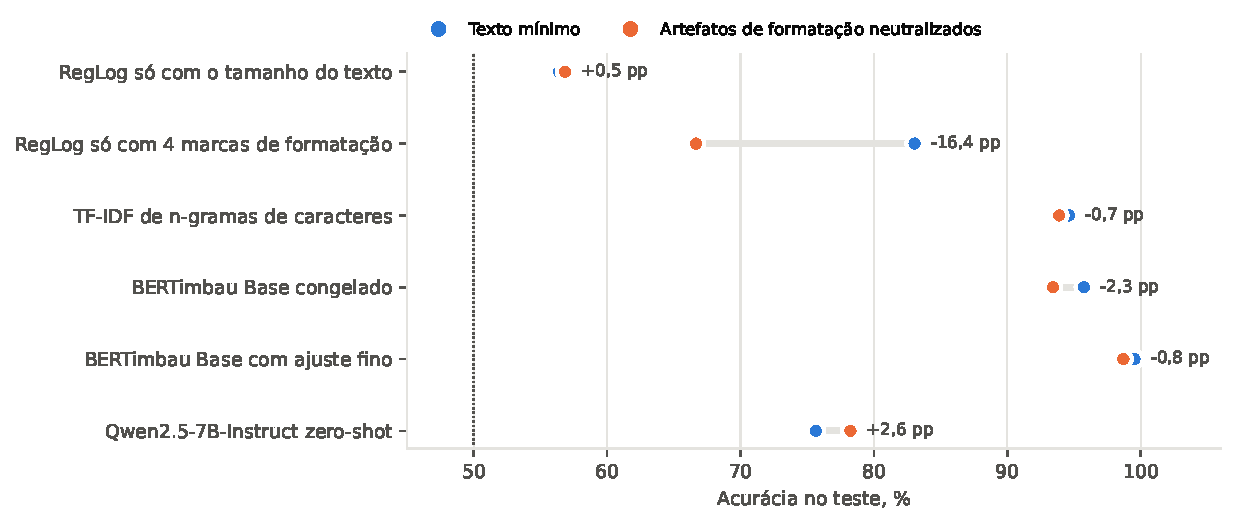
\includegraphics[width=0.85\textwidth]{figuras/robustez_artefatos.pdf}
\caption{Acurácia de cada modelo no texto mínimo e com os artefatos de formatação neutralizados.}
\label{fig:robustez}
\end{figure*}

A neutralização (Tabela~\ref{tab:robustez}, Figura~\ref{fig:robustez}) quase não afeta os n-gramas de caracteres ($-0{,}7$ ponto, não significativo), custa 0,8 ponto ao BERTimbau ajustado, que mantém 98,7\% $\pm$ 0,3, e 2,3 pontos aos embeddings congelados. A análise por subgrupo (Tabela~\ref{tab:final}) mostra por quê: nas verdadeiras que terminam com pontuação, contrárias ao atalho, o BERTimbau congelado e o E5 caem para 80,6\%, enquanto o BERTimbau ajustado mantém 98,2\% e 96,8\% nos dois subgrupos contrários ao atalho.

O LLM tem o comportamento oposto: \textbf{melhora} 2,6 pontos com a neutralização. Ele não explora o atalho; ao contrário, é prejudicado por ele. As notícias verdadeiras truncadas no meio da frase lhe parecem suspeitas: acerta só 72,7\% delas, contra 93,5\% das verdadeiras completas, e a neutralização eleva esse subgrupo a 82,1\%.

\begin{table*}[t]
\centering\small
\begin{adjustbox}{max width=\textwidth}
\begin{tabular}{llrcccccc}
\toprule
Classe & Final do texto & $n$ & SVM & Caracteres & BERTimbau cong. & E5 & BERTimbau ajust. & Qwen \emph{zero-shot} \\
\midrule
Falsa & com pontuação & 371 & 91,4 & 92,5 & 96,0 & 90,6 & 100,0 & 75,2 \\
\emph{Falsa} & \emph{sem pontuação} & 169 & 92,3 & 94,1 & 92,3 & 91,7 & 98,2 & 82,2 \\
\emph{Verdadeira} & \emph{com pontuação} & 31 & 93,5 & 96,8 & 80,6 & 80,6 & 96,8 & 93,5 \\
Verdadeira & sem pontuação & 509 & 91,6 & 96,3 & 97,6 & 92,1 & 100,0 & 72,7 \\
\bottomrule
\end{tabular}
\end{adjustbox}
\caption{Acurácia (\%) por classe e por final do texto original. Em itálico, os subgrupos contrários ao atalho (falsa truncada, verdadeira completa). BERTimbau ajustado: semente 42; Qwen com limiar calibrado.}
\label{tab:final}
\end{table*}

\subsection{Custo}

O ajuste dos modelos estatísticos, incluindo a validação cruzada, leva de 1 a 36~s em CPU, e a inferência menos de 1~ms por notícia. Os embeddings congelados exigem GPU para codificar o corpus (1 a 3~min) e cerca de 10 a 25~ms por notícia. O ajuste fino do BERTimbau leva de 6 a 10~min por semente, com cerca de 6~ms por notícia. O LLM não tem custo de treino, mas é o mais caro na inferência: 0,26~s por notícia em \emph{zero-shot} e 1,1~s em \emph{few-shot}, de 40 a 190 vezes o BERTimbau ajustado.

% ============================================================================================
\section{Análise de Erros}

\begin{table*}[t]
\centering\small
\begin{adjustbox}{max width=\textwidth}
\begin{tabular}{lrccccccc}
\toprule
Notícias falsas de\ldots & $n$ & NB & SVM & Caracteres & BERTimbau cong. & BERTimbau ajust. & BERTimbau ajust. (neutro) & Qwen \emph{zero-shot} \\
\midrule
diariodobrasil.org & 496 & 88,9 & 94,2 & 96,0 & 96,6 & 100,0 & 98,4 & 77,8 \\
outras 5 fontes & 44 & 56,8 & 63,6 & 59,1 & 75,0 & 93,2 & 97,7 & 72,7 \\
\bottomrule
\end{tabular}
\end{adjustbox}
\caption{Revocação da classe falsa (\%) por origem da notícia falsa. BERTimbau ajustado: semente 42; Qwen com limiar calibrado.}
\label{tab:fonte}
\end{table*}

\paragraph{Por fonte.} Para os modelos estatísticos e os embeddings congelados, a revocação cai de 22 a 37 pontos fora do site dominante (Tabela~\ref{tab:fonte}): boa parte do seu desempenho vem de reconhecer o estilo de um único site. O BERTimbau ajustado é a exceção, com 93,2\%, e chega a 97,7\% no texto neutro: os poucos erros que cometia nas fontes minoritárias vinham do atalho do truncamento. O LLM, que não foi treinado no corpus, tem desempenho baixo, mas parecido nos dois grupos (77,8\% e 72,7\%). A amostra de outras fontes é pequena (44 notícias), mas a diferença é grande e consistente.

\paragraph{Por categoria e tamanho.} O desempenho é homogêneo entre as três categorias maiores; economia e religião têm poucas notícias de teste (12 e 6). Nos modelos estatísticos e congelados, a acurácia cai no quartil das notícias mais longas (de 97,0\% para 91,4\% no BERTimbau congelado), enquanto o BERTimbau ajustado fica acima de 99\% em todos os quartis.

\paragraph{Erros do BERTimbau ajustado.} Os poucos erros se repetem entre as sementes e são quase todos casos contrários aos atalhos: notícias falsas de fontes minoritárias que eram a mais longa do par e foram truncadas no meio da frase; um texto de tom satírico de um site de comentário político; e notícias verdadeiras de gênero não noticioso, como uma coluna de opinião em primeira pessoa. Nenhuma notícia de teste é errada por todos os oito modelos principais. Sátira e opinião não se acomodam bem em ``falsa'' e ``verdadeira''.

% ============================================================================================
\section{Discussão}

No Fake.Br normalizado, o BERTimbau ajustado é claramente superior: 99,5\% de acurácia, 98,7\% sem os artefatos de formatação e o único que generaliza para as fontes minoritárias, com custo modesto (minutos de GPU no treino, milissegundos por notícia). Os n-gramas de caracteres com SVM são a melhor opção sem GPU (94,6\%, robustos aos artefatos), e o TF-IDF de palavras segue útil pela interpretabilidade. Os embeddings congelados não compensam: igualam os n-gramas de caracteres com custo maior e dependem mais dos atalhos. O LLM dispensa treino e não aprende os atalhos do corpus, mas fica 10 a 21 pontos abaixo dos modelos treinados e custa de 40 a 190 vezes mais por notícia; exemplos no \emph{prompt} e calibração do limiar ajudam, mas não fecham a distância.

O desempenho no Fake.Br não deve ser lido como capacidade de detectar desinformação em geral: parte considerável pode ser obtida sem ler o conteúdo, e os modelos mais simples dependem fortemente do estilo de um único site. Recomendamos que trabalhos futuros no corpus usem a versão normalizada com neutralização do final dos textos, particionem por par e reportem o desempenho por fonte.

\paragraph{Limitações.} As notícias falsas vêm de poucos sites e de 2016--2018, e a avaliação fora do site dominante usa só 44 notícias; uma avaliação com fontes disjuntas (\emph{leave-source-out}) não foi possível. O corpus é público desde 2018 e pode ter contaminado o pré-treinamento do LLM. Avaliamos um único LLM e um único \emph{prompt}, e o \emph{few-shot} só no texto mínimo. Sátiras, opiniões e textos parcialmente verdadeiros não se acomodam num rótulo binário. Alguns experimentos dividiram a GPU, então os tempos são aproximados.

% ============================================================================================
\section{Conclusão}

Comparamos quatro famílias de modelos para detecção de notícias falsas em português sob um protocolo reprodutível. O BERTimbau com ajuste fino atingiu 99,5\% de acurácia e foi o único a manter o desempenho fora do site dominante e nos casos contrários aos atalhos; n-gramas de caracteres com SVM são a melhor alternativa sem GPU; e o LLM por aprendizado no contexto, embora dispense treino, ficou em 78,4\% no melhor cenário. O resultado mais importante, porém, é metodológico: o Fake.Br contém atalhos de tamanho, de formatação (criados pela própria normalização) e de fonte, capazes de produzir acurácias altas sem relação com a veracidade. Trabalhos futuros incluem avaliar em notícias de outras fontes e períodos, construir partições com fontes disjuntas e usar técnicas de explicação para verificar em que partes do texto o BERTimbau se apoia.

% Opcional (seção sem número, como no modelo):
% \section*{Agradecimentos}
% Texto dos agradecimentos.

\bibliographystyle{sp_por}
\bibliography{referencias}

\end{document}
